\section{Инструкции по установке даты запрета редактирования документов 1С Розница}

\subsection{Настройка даты запрета}

\begin{itemize}
	\item Для возможности гибкого управления запретом редактирования документов прошлых периодов в 1С Розница предусмотрена гибкая настройка.
\end{itemize}	
\begin{enumerate}	
	\item Настройка даты запрета редактирования находится в разделе:\par 
	\menu[,]{Администрирование,Поддержка и обслуживание,Регламентные операции}
	 Рис.~\ref{ris:1.jpg}
	\begin{figure}[H]
		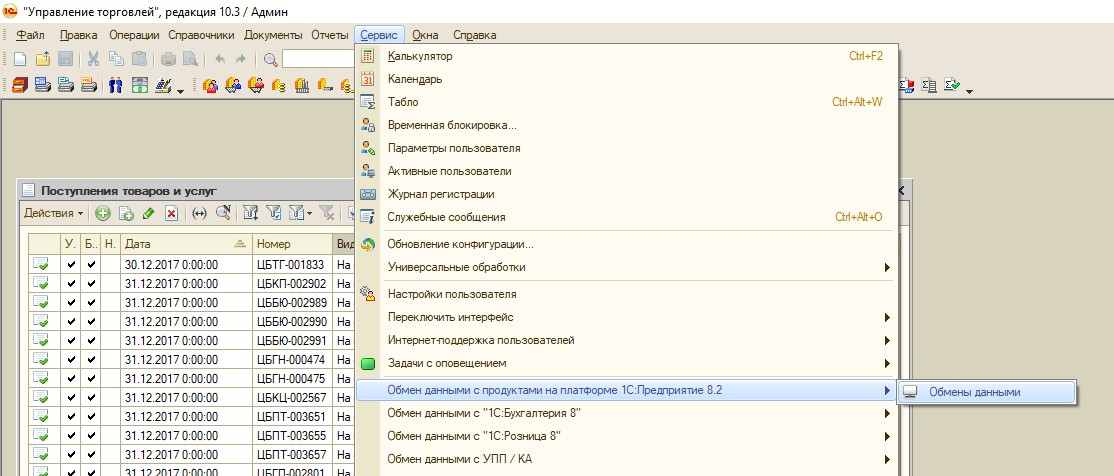
\includegraphics[width=0.7\textwidth]{1.jpg}
		\caption{Расположение в разделе ,,Администрирование``.}
		\label{ris:1.jpg}
	\end{figure}
	\begin{figure}[H]
	
		\caption{Расположение в разделе ,,Поддержка и обслуживание``.}
		\label{ris:2.jpg}
	\end{figure}
	\begin{figure}[H]
		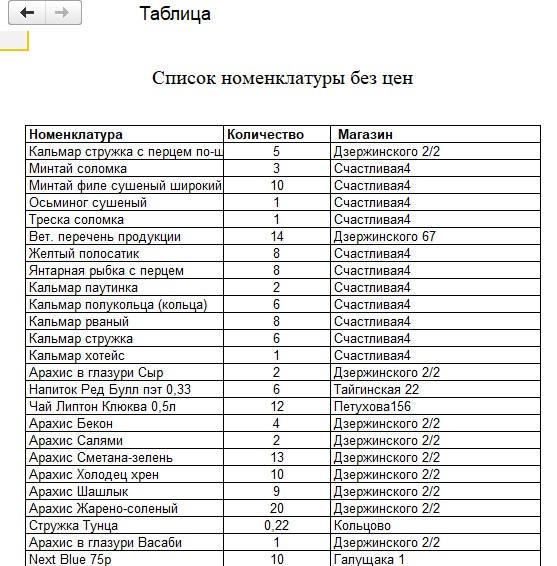
\includegraphics[width=0.7\textwidth]{3.jpg}
		\caption{Расположение в разделе ,,Регламентные операции``.}
		\label{ris:3.jpg}
	\end{figure}
	


	\item Далее выбираем пункт ,,Настроить`` напротив "<Дата запрета редактирования"> Рис.~\ref{ris:3.jpg}
	
	\item Открывается форма настройки даты запрета редактирования Рис.~\ref{ris:4.jpg}
	\begin{figure}[H]
		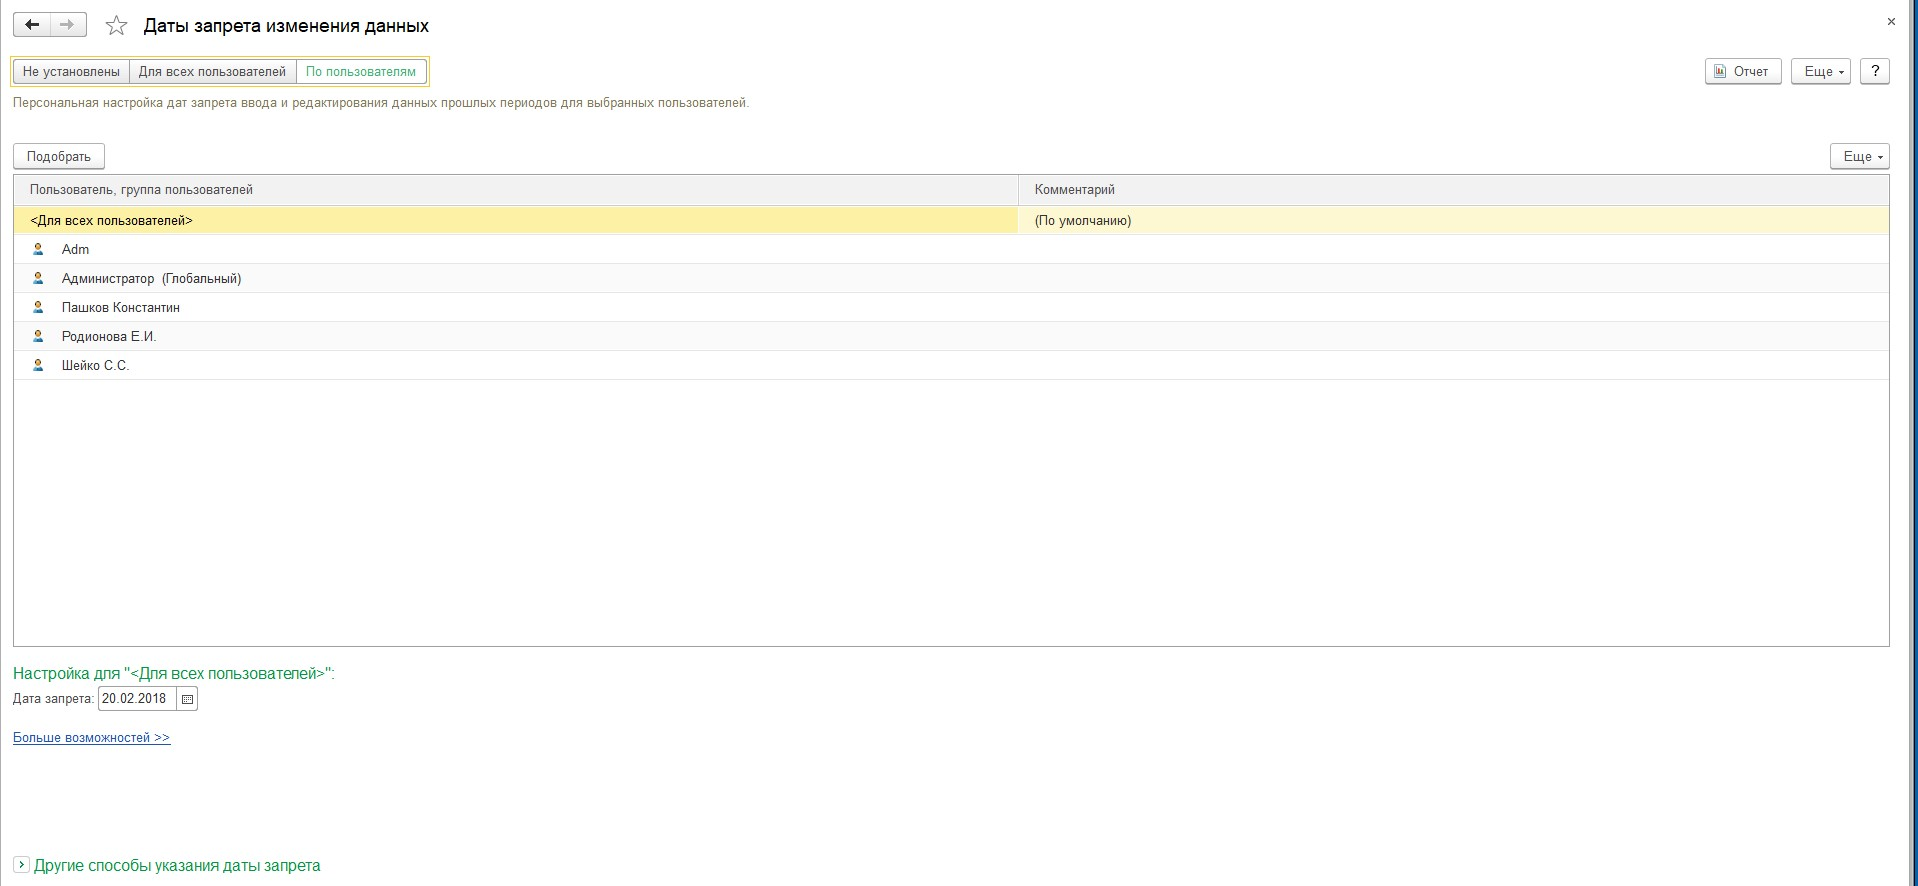
\includegraphics[width=0.7\textwidth]{4.jpg}
		\caption{,,Настройка даты запрета редактирования``.}
		\label{ris:4.jpg}
	\end{figure}

	\item В таблице выбираем пользователя или группу пользователей для которой мы хотим установить дату запрета редактирования. Слева внизу раскрываем пункт "<Другие способы указания даты запрета"> Рис.~\ref{ris:5.jpg}
	\begin{figure}[H]
		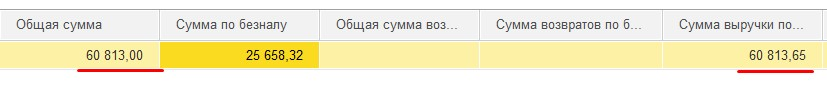
\includegraphics[width=0.7\textwidth]{5.jpg}
		\caption{,,Выбор пользователя``.}
		\label{ris:5.jpg}
	\end{figure}\par \par 

	\item В пункте "<Другие способы указания даты запрета"> из выпадающего списка нужно выбрать "<По разделам и объектам"> Рис.~\ref{ris:6.jpg}
	\begin{figure}[H]
		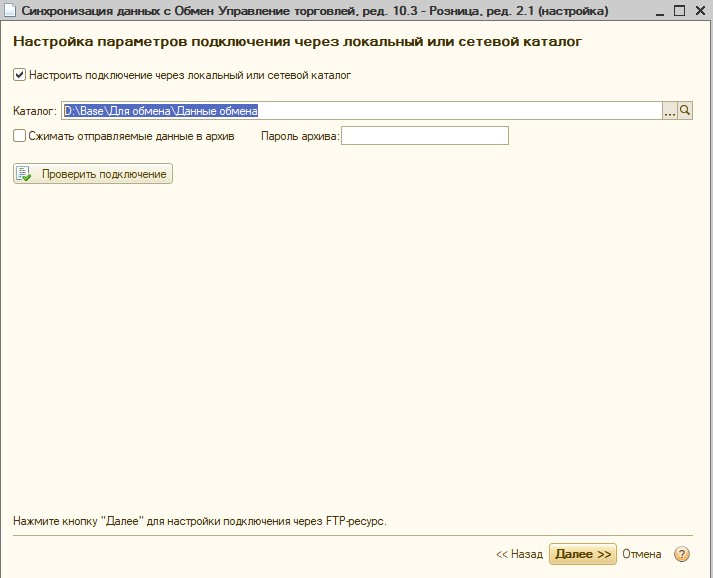
\includegraphics[width=0.7\textwidth]{6.jpg}
		\caption{,,Выбор способа указания``.}
		\label{ris:6.jpg}
	\end{figure}

	\item В выбора пункта "<По разделам и объектам"> появляется дополнительная табличная часть Рис.~\ref{ris:7.jpg}
	\begin{figure}[H]
		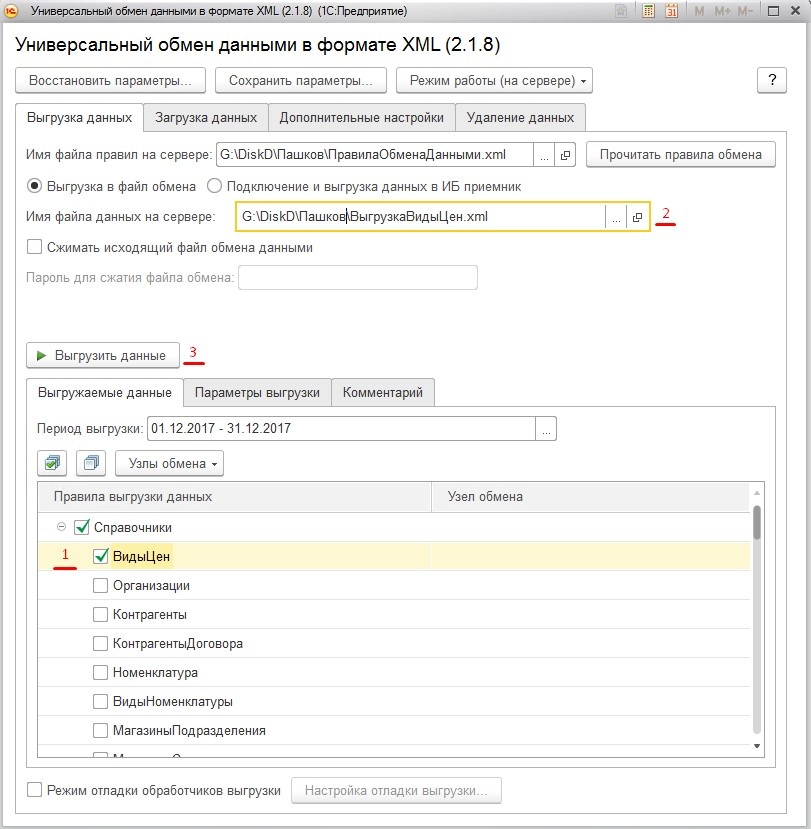
\includegraphics[width=0.7\textwidth]{7.jpg}
		\caption{,,Табличная часть для тонкой настройки``.}
		\label{ris:7.jpg}
	\end{figure}

	\item Для настройки разных дат запрета по магазинам и пользователям необходимо: Рис.~\ref{ris:8.jpg}
	\begin{enumerate}	
		\item Выделить в табличной части "<Учет по магазинам">
		\item Нажать кнопку \keys{Подобрать}
			\begin{figure}[H]
				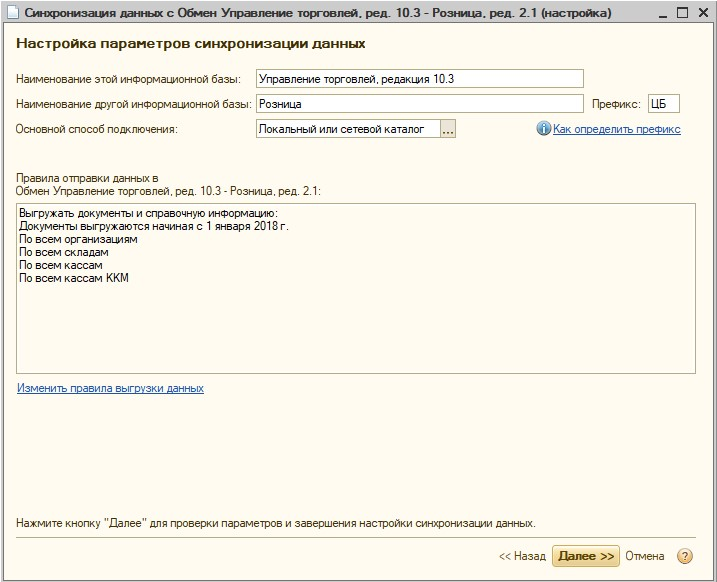
\includegraphics[width=0.7\textwidth]{8.jpg}
				\caption{,,Настройка``.}
				\label{ris:8.jpg}
		\end{figure}
		\item Далее двойным кликом по выбранной строке или нажатием кнопки \keys{Выбор} переносим один или несколько магазинов в табличную часть Рис.~\ref{ris:9.jpg}
		\begin{figure}[H]
			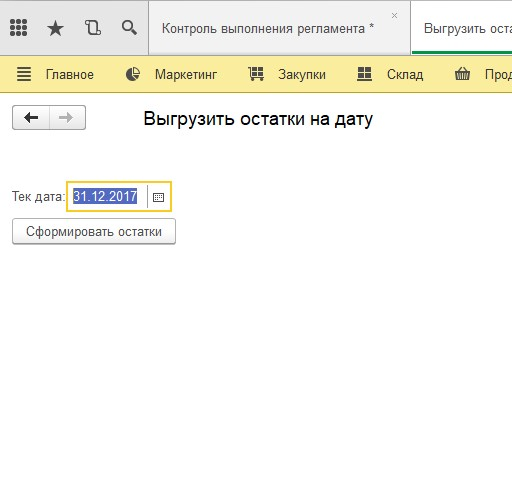
\includegraphics[width=0.7\textwidth]{9.jpg}
			\caption{,,Выбор магазина``.}
			\label{ris:9.jpg}
		\end{figure}
		\item После того как все магазины выбраны закрываем форму выбора Рис.~\ref{ris:10.jpg}
		\begin{figure}[H]
			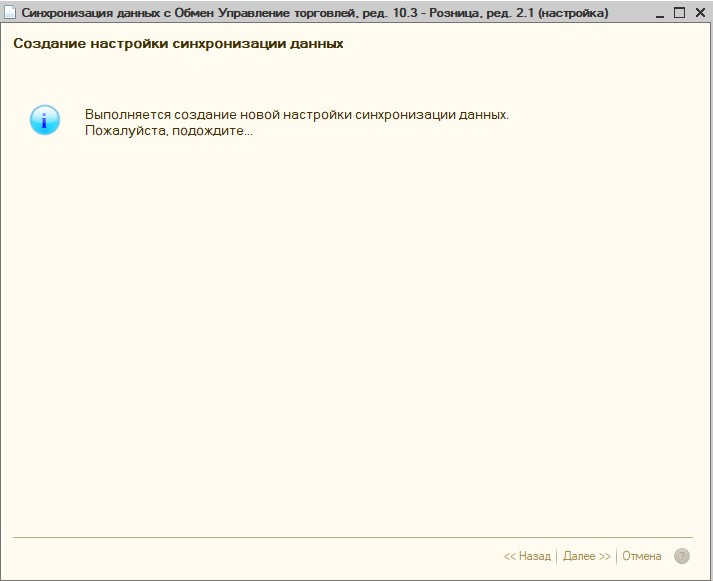
\includegraphics[width=0.7\textwidth]{10.jpg}
			\caption{,,Магазины выбраны``.}
			\label{ris:10.jpg}
		\end{figure}
	\item Далее для каждого магазина указываем нужную дату запрета Рис.~\ref{ris:11.jpg}
		\begin{figure}[H]
			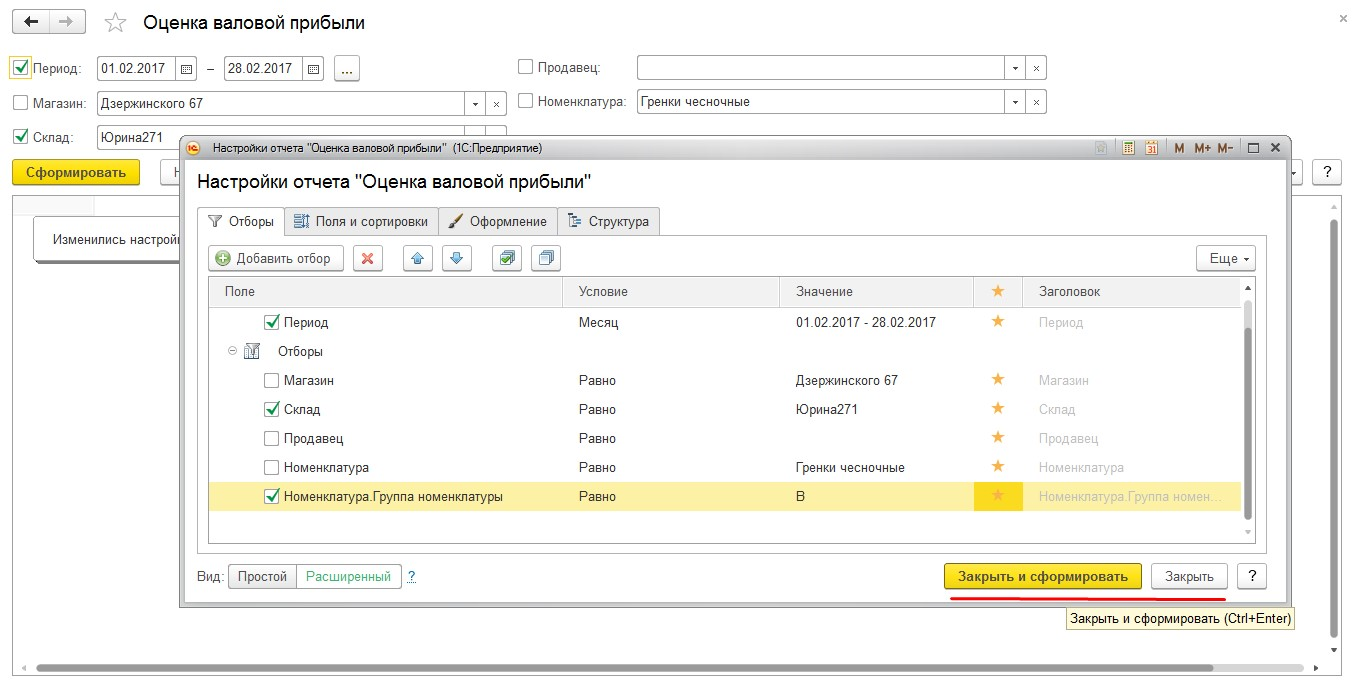
\includegraphics[width=0.7\textwidth]{11.jpg}
			\caption{,,Установленные даты запрета по магазинам``.}
			\label{ris:11.jpg}
		\end{figure}
	\end{enumerate}

	\item Данную операцию можно проводить как в Центральном узле, так и в магазинах. Например можно установить по магазину "<Кропоткина"> <Для всех пользователей> дату запрета 10.03.2018, а для Пользователя "<Родионова"> дату запрета 01.02.2018

	\end{enumerate}

